\documentclass[12pt,twoside,a4paper]{report}
%\usepackage[utf8x]{inputenc}
\usepackage{natbib}
\usepackage{a4wide}
\usepackage{graphicx}
\usepackage{amsmath}
\usepackage[cm]{fullpage}
\usepackage{hyperref}
\usepackage{coffee4}
\frenchspacing
%opening
\title{Users Guide to the UCT 14 Inch telescope}
\author{Thuso Simon \\
	thuso@ast.uct.ac.za \\
	Version $0.1$}


\begin{document}

\maketitle
\tableofcontents

\chapter{Introduction}
Welcome to the 14 Inch telescope. This is a modern telescope that is used for teaching and simple astronomy projects. This guide will help to get you understand and use without breaking the telescope.

Right now this guide will only cover how to do photometry, but in the future it will include spectroscopy as well.
\chapter{Basic Observation Procedures}
If you want to get started at making images quickly and don't have the time to get into the nitty gritty details of astronomy go to the next section.

\subsection{Start of Night Check List}
\begin{enumerate}
 \item Plug in observation computer to power, Internet, Dome controller usb and Telescope controller usb and turn on switches in observatory.
 \item Take off telescope cover and open dome.
 \item Put telescope mount from lock to star position on both RA and Dec controllers.
 \item Start \emph{TheSkyX} and \emph{Maxim DL} if \emph{TheSkyX} cannot use the CCD.
 \item Connect observation computer to Internet if wanting to use remote software (see \ref{remote_obs} for more information). 
 \item Make sure chairs and tables are not in the way telescopes movement.
 \item Connect dome control, rotation and mount control in \emph{TheSkyX}. Tell all to go to home position and start! See section \ref{Dome_control} for more information.
 \item Find star to focus (less than 7.5 - 9 magnitude star) using Focus Max.
 \item Fine tune dome position (see section \ref{dome_position}).
 \item Slew to object, select filter, check rotation and expose and get some coffee.
 
\end{enumerate}

%coffee stain
\cofeAm{.1}{1.0}{0}{5.5cm}{3cm}

\subsection{End of Night Check List}
\begin{enumerate}
 \item Park telescope and Dome and disconnect all systems from computer.
 \item Turn off observation computer.
 \item Put mount from star position to lock position.
 \item Power off all power supplies in dome.
 \item Close the dome shutter.
 \item Put telescope cover over telescope.
 \item Get some sleep.
\end{enumerate}

\subsection{\emph{The SkyX}}

\begin{figure}[h]
 \centering
    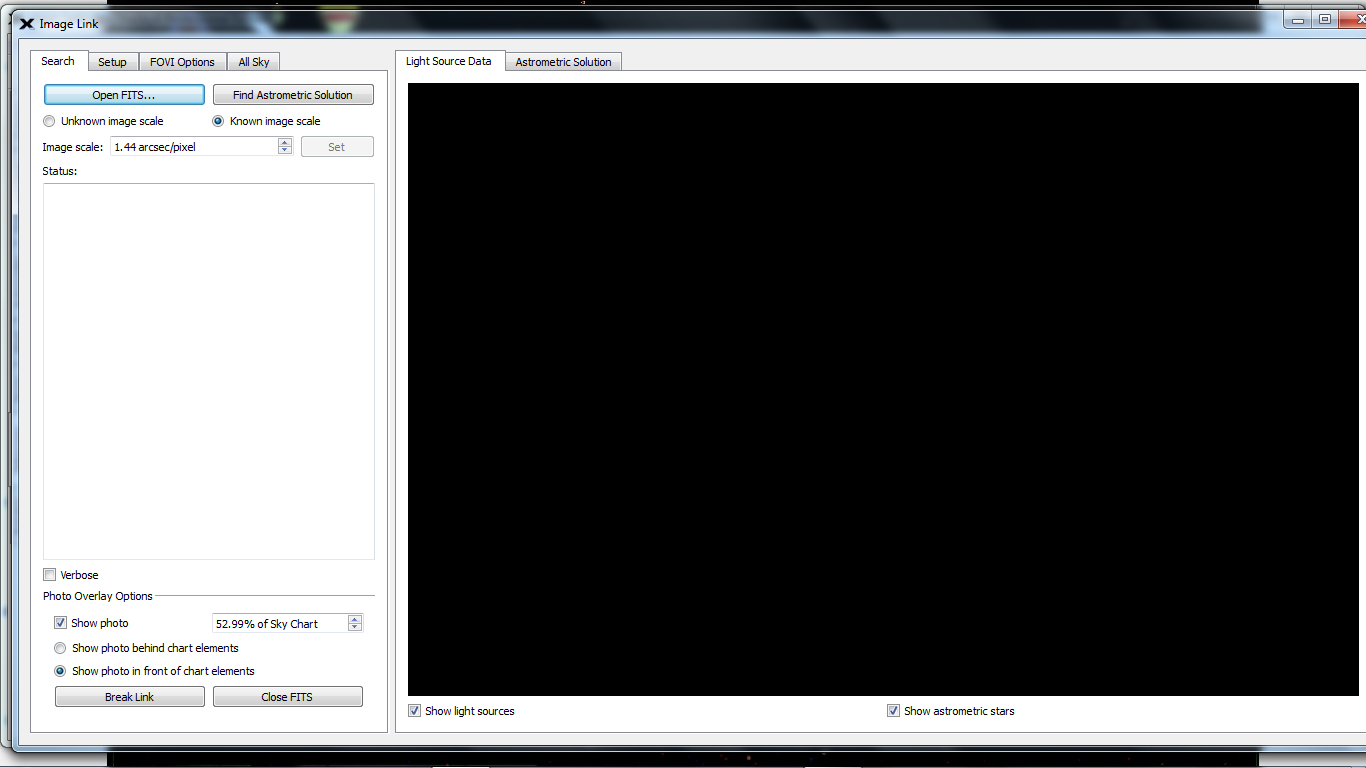
\includegraphics[width=\textwidth]{documentation_images/basic_interface.png}
    \caption{\label{fig:basic_interface} This is how \emph{The SkyX} looks like when it is open.}
\end{figure}

\emph{TheSkyX} is an all inclusive astronomy program, that gives you the power of the universe at the point of a mouse. It is should be able to guide the telescope, control the CCD, Focus the image, control the dome and control the rotator. Unfortunately, it has some bugs so all it can really control is the telescope mount and sometimes the CCD. Fortunately, We have come up with workarounds for most of the bugs that have been seen in the sky. To access the user manual for the sky, which is better written and highly recommended, visit \url{http://www.bisque.com/help/TheSkyXSAEAndPro/index.htm}.

\subsection{Starting the \emph{The SkyX}}
Once \emph{The SkyX} is open, you will need to connect it to the components that you would like it to control. To connect it to the mount, click on the Telescope tab on the left and the select the start up tab. Select connect telescope and then \emph{Find Home}. This will allow you to properly initialize the telescope and give it a better chance at having good pointing right away. See figure \ref{fig:connect_telescope} to see what the menu looks.

\begin{figure}[h]
 \centering
    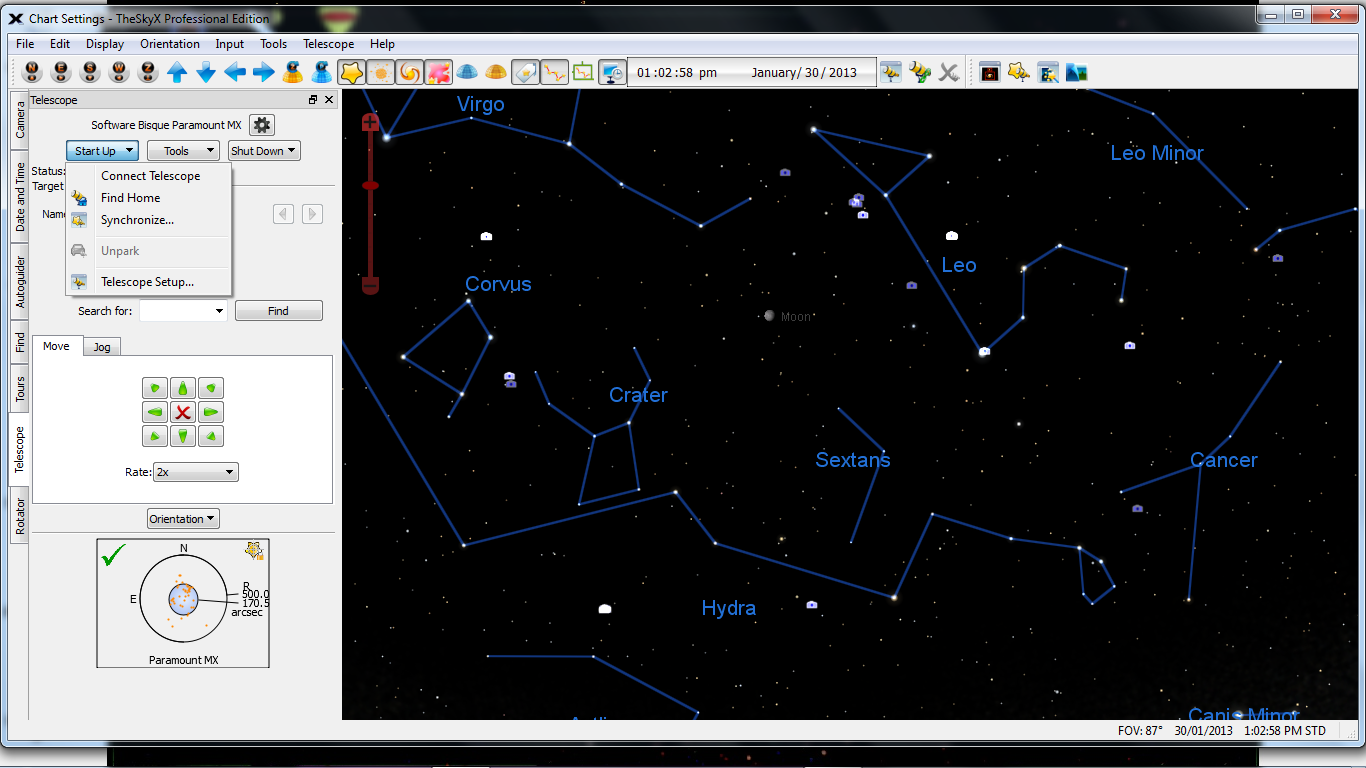
\includegraphics[width=\textwidth]{documentation_images/connect_telescope.png}
    \caption{\label{fig:connect_telescope} Shows how to connect the computer to the telescope.}
\end{figure}

\subsubsection{Small Changes to Pointing}
\label{small_changes_to_pointing}
If the pointing of the telescope is off, follow these steps to correct it.
\begin{enumerate}
 \item Slew to field you would like to be look at.
 \begin{figure}[h]
 \centering
    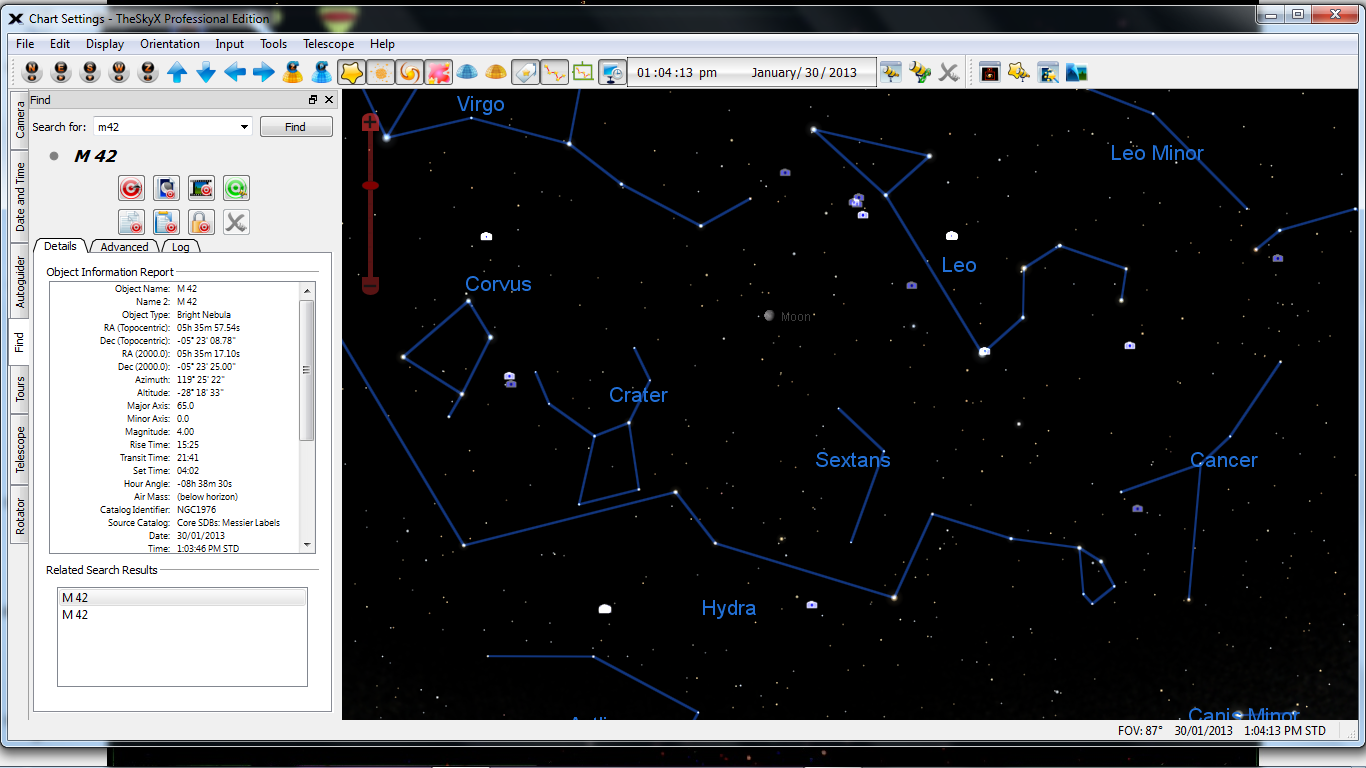
\includegraphics[width=\textwidth]{documentation_images/moving_telescope.png}
    \caption{\label{fig:moving_telescope} Click the green slew button to start the telescopes movement.}
\end{figure}
 \item \label{2} Take an image with your favorite CCD manager and save it.
 \item In \emph{The SkyX}, under the menu tools--Image link (Ctrl+Shift+I), in the Search tab, click the \emph{Open FITS...} window.
  \begin{figure}[h]
 \centering
    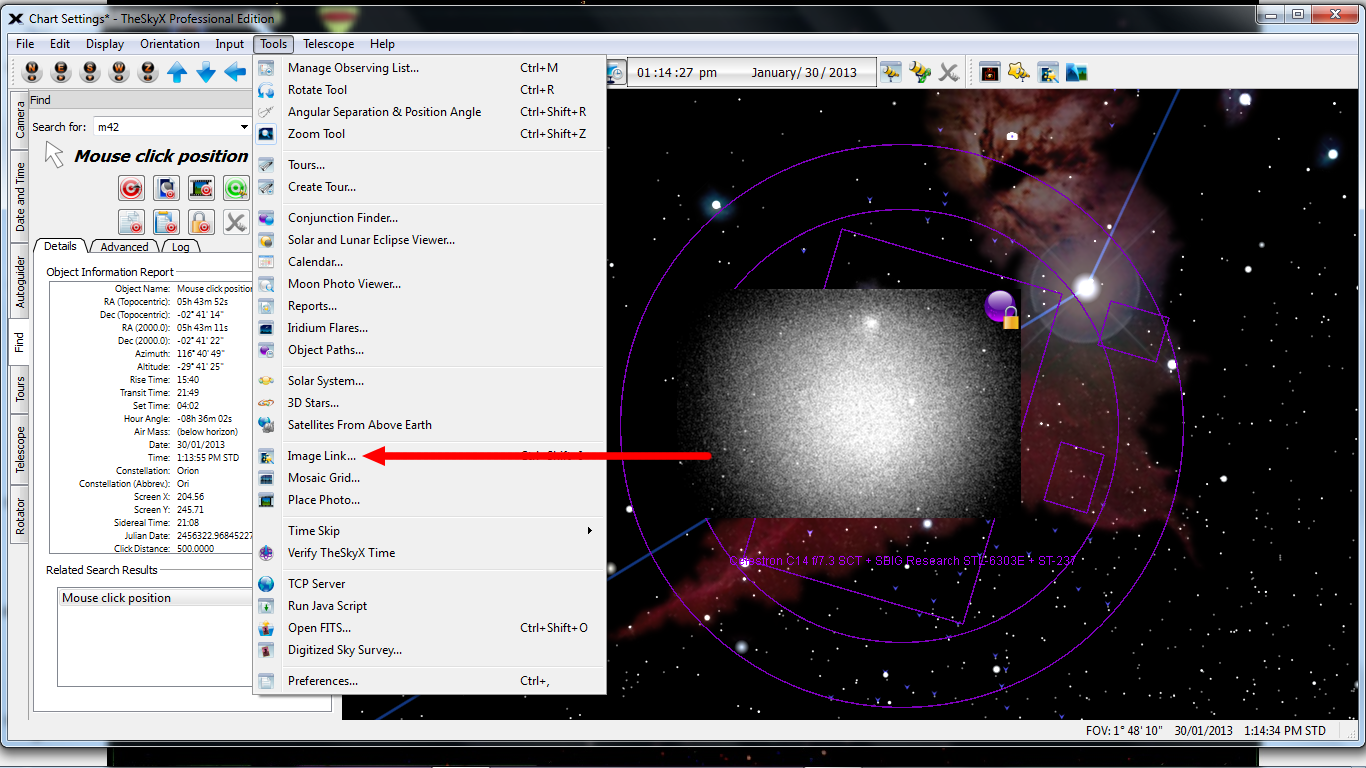
\includegraphics[width=\textwidth]{documentation_images/tools_menu_1_1.png}
    \caption{\label{fig:tools_menu} Click at arrow to access image linking window.}
    \end{figure}
    
  \begin{figure}[h]
 \centering
    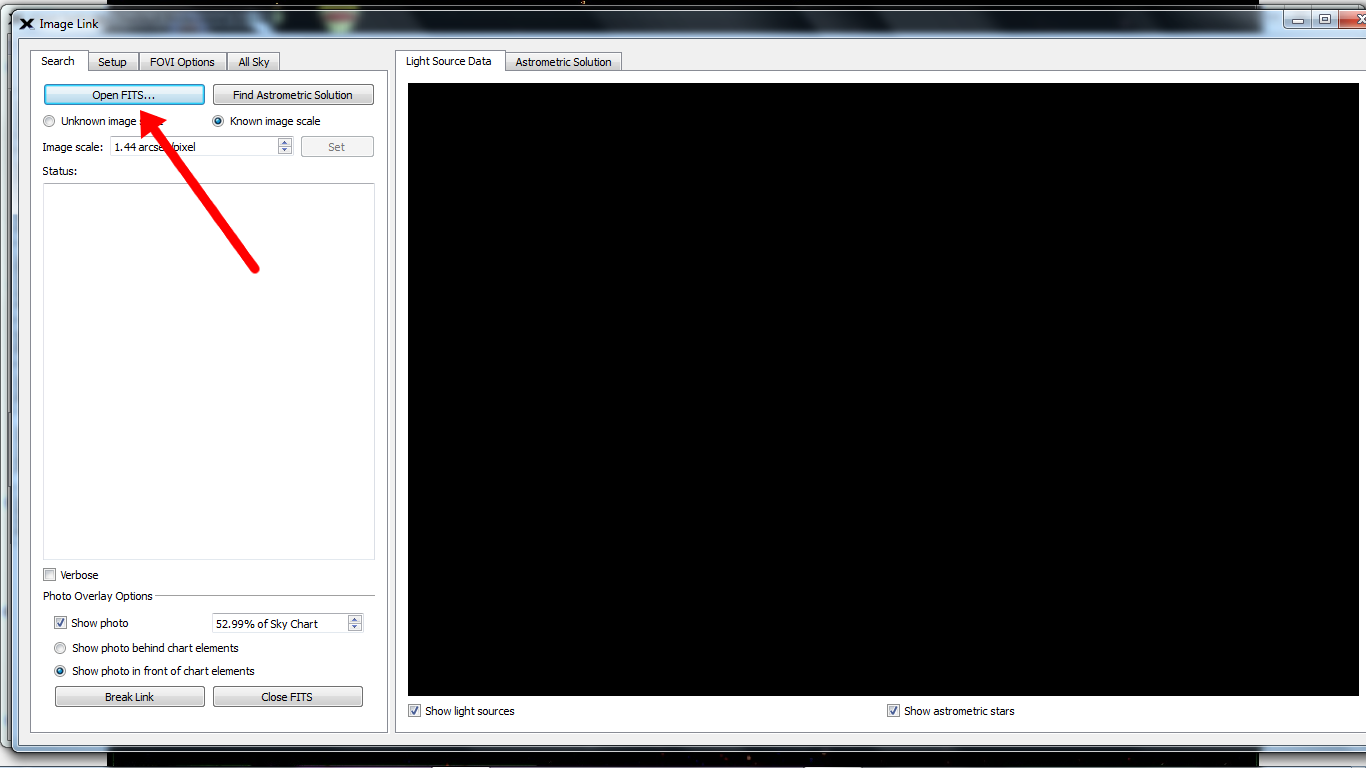
\includegraphics[width=\textwidth]{documentation_images/pointing1_1.png}
    \caption{\label{fig:pointing1} Click at arrow to access image linking window.}
    \end{figure}

 \item Load in saved test field from step \ref{2} and then click the \emph{Find Astrometric Solution} button.
 \item If solution fails, check Image scale and binning of image they should be:
 \begin{itemize}
  \item $1\times1 = 0.72$ arcseconds
  \item $2\times2 = 1.44$ arcseconds
  \item $3\times3 = 2.15$ arcseconds
  \item $4\times4 = 2.88$ arcseconds 
 \end{itemize}
 \item Go to the \emph{FOVI Options} tab and click the \emph{Synchronize Rotator Angle to Position Angle} button.
  \begin{figure}[h]
 \centering
    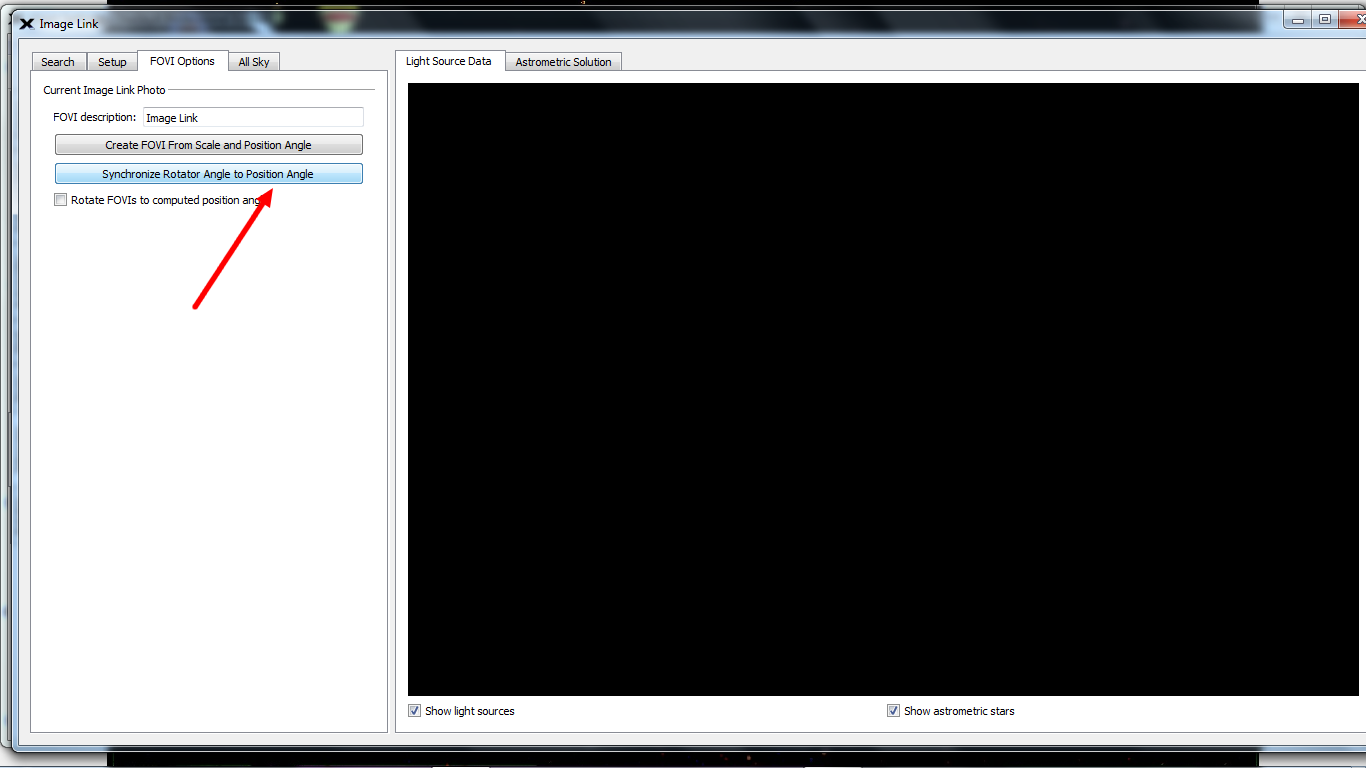
\includegraphics[width=\textwidth]{documentation_images/pointing2_1.png}
    \caption{\label{fig:pointing1} Click at arrow to access sync telescope pointing with image.}
    \end{figure}

 \item Exit from window and go back to the main screen.
 \item Click on Image until in the \emph{Find} tab shows Linked Photo.
 \item Click on the \emph{Sync} button on the tool-bar and it should be pointing in the correct direction now. If not repeat from beginning.
\end{enumerate}

\subsubsection{Rotator}
\label{Correcting_rotation}
\emph{The SkyX} can control the rotation of the camera, but there is a bug in the software that causes the readings to be off, and this changes depending on where you are pointing in the sky. There is also no easy way to adjust the rotation of the CCD in \emph{The SkyX}.

The rotator is important for selecting a guide star for the Adaptive Optics (AO). The following steps tell you how to calibrate and align a guide star on the AO CCD.
\begin{enumerate}
 \item 
\end{enumerate}


\subsubsection{Remote Observations}
\label{remote_obs}
Sitting in the dome all night while the telescope integrates isn't a good idea. The temperature differences between your body can cause differences in the seeing in the telescope. We have set up a way to access the telescope computer from a remote place, so that the disturbances of the telescope are kept to a minimum.

To get the remote control software, goto \url{http://www.teamviewer.com/en/} and install the software on your computer. To access the observatory computer use the address: telescope.ast.uct.ac.za and password: Bonjour7.

Make sure that in the observatory that the telescope wont run into anything as it move throughout the night. Sit back in your remote setting and keep and eye out for rain, too much wind and relax!

\subsubsection{Dome Control}
\label{Dome_control}
TBA
\label{dome_position}

\section{Maxim DL}
\subsubsection{Adaptive Optics}

\subsubsection{Dome Control}

\subsubsection{Camera Control}

\subsubsection{Setting up Batch Mode for Images}


\chapter{Advanced Observation Procedures}

\chapter{Switching Instruments}

\chapter{Maintenance}

\chapter{Using Maxim DL for Imaging and Science}

\appendix
\chapter{A}

\end{document}
